\chapter{Analiza dziedzinowa}
Niniejsza praca wiąże się z teorią muzyki. Przy pierwszym spotkaniu teoria ta może wydawać się mało zrozumiała. Dlatego postanowiono przybliżyć ją czytelnikowi wyjaśniając znaczenie wybranych konceptów i terminów.
\section{Podstawy teoretyczne}
Na początek wyjaśnić należy czym są \emph{skale muzyczne}, pojawiające się one w wielu częściach tworzonej aplikacji. Skala muzyczna, mówiąc w skrócie, to zestaw nut, które zagrane w połączeniu ze sobą dają dźwięk postrzegany przez ludzki mózg jako przyjemny. Skala durowa i~molowa (obsługiwane w aplikacji) składają się z 7 dźwięków. Do zobrazowania obu tych skal wykorzystuje się \emph{koło kwintowe} jak na rysunku~\ref{fig:kolokwintylowe}. 
\begin{figure}[htb]
	\centering
	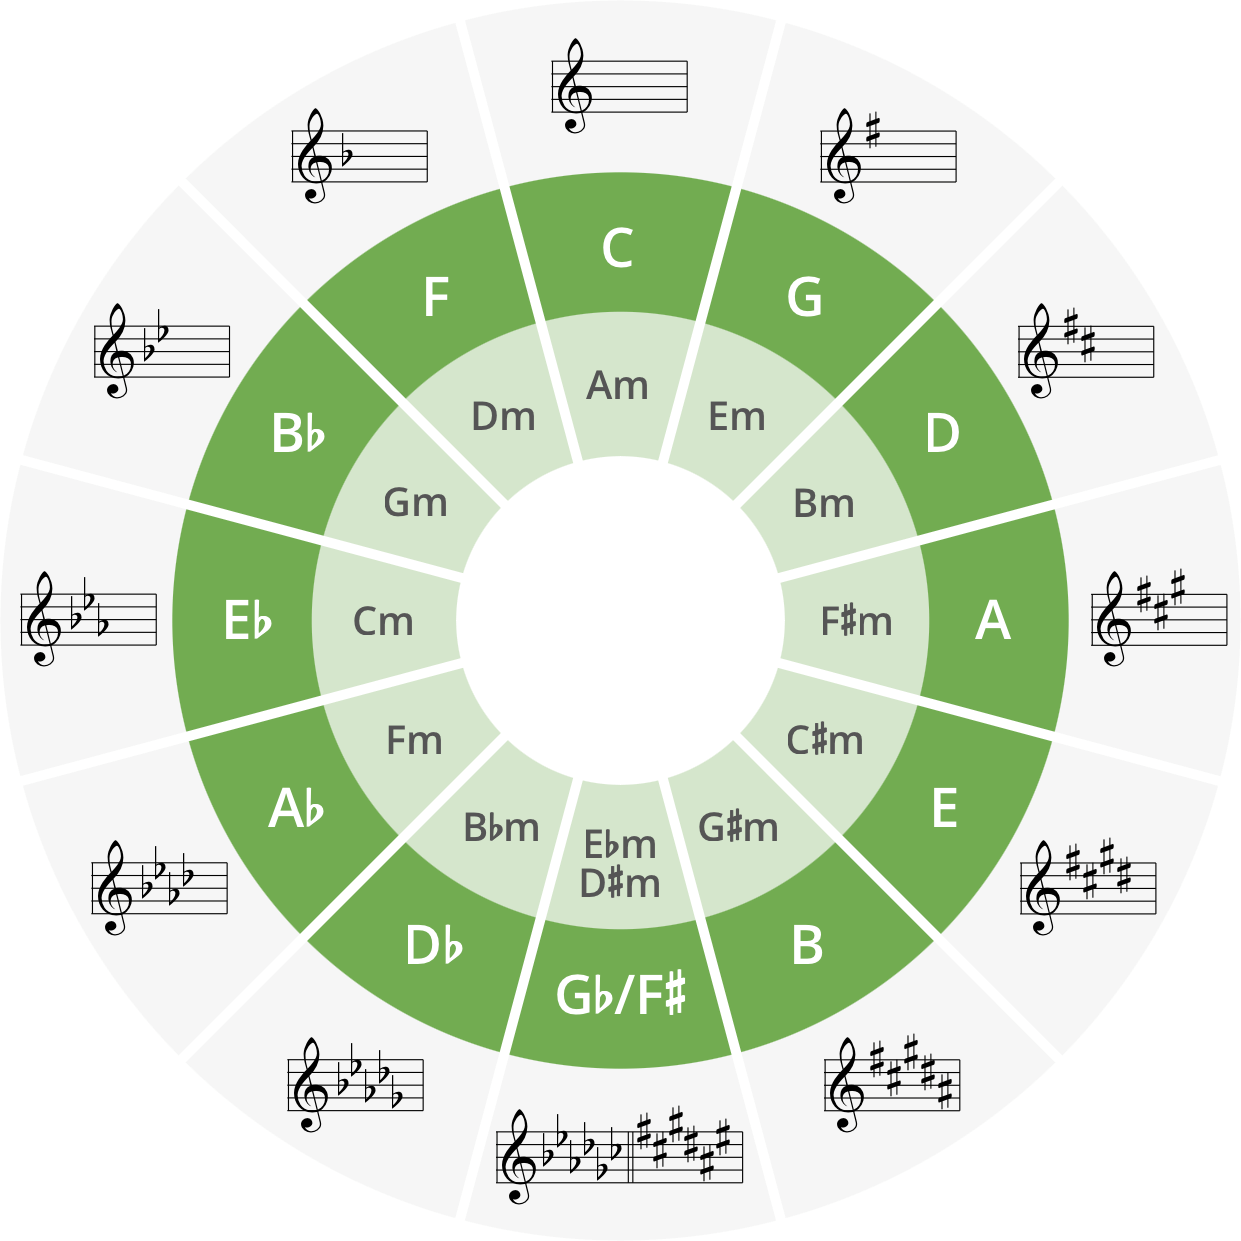
\includegraphics[width=.48\linewidth]{rys02/cof2.1}
	\caption{Wizualizacja koła kwintowego} \label{fig:kolokwintylowe}
\end{figure}

Koło kwintowe reprezentuje nuty ułożone na okręgu, przy czym nie są one ułożone według klasycznego zestawienia -- skali chromatycznej (C, C\#, D, D\#, E, F, F\#, G, G\#, A, A\#, B -- jedna gama dźwięków, odpowiadająca kolejnym klawiszom pianina), lecz za pomocą naturalnego ułożenia dźwięków. 
Przez naturalne ułożenie dźwięków należy rozumieć różnice pomiędzy częstotliwościami poszczególnych nut, na kole kwintowym są one ułożone w kolejności rosnącej, dzięki temu można w łatwy sposób dostrzec skąd biorą się poszczególne skale. Takie koło zostanie zaimplementowane jako jedna z funkcji autorskiej aplikacji.


Ważnym narzędziem dla muzyków jest metronom. Urządzenie to służy do wybijania rytmu, użytecznego przy okazji treningu słuchu oraz wyczuwania owego rytmu podczas gry. 
% DONE: w zaleceniach było, jak pisać agielskojęzyczne terminy !!!!!
Wymijanie rytmu można parametryzować. Określa się np.\ parametr bpm (ang.~\emph{beat per minute}) -- liczba uderzeń na minutę. Ponadto zwykle możliwe jest wybranie jednej z 4 opcji wyboru wybijania rytmu, bazujące na 4 podstawowych nutach. Są to: cała nuta -- jedno uderzenie na takt, pół nuta -- dwa uderzenia na takt, ćwierć nuta -- trzy uderzenia na takt, ósemka -- 4 uderzenia na takt. Działanie metronomu polega na wybijaniu poszczególnych taktów, podążając za ustalonym wcześniej tempem gry. 

Jeżeli chodzi o notację gitarową, to podczas realizacji niniejszej pracy posłużono się najbardziej rozpowszechnioną i czytelną formą. Do reprezentacji akordów (zbiorów nut, które grane ze sobą tworzą ujednolicony dźwięk) posłużono się widokiem gryfu gitarowego, przy czym czytając od góry reprezentowana jest kolejno 1, 2, 3, 4, 5, 6 struna gitary. Obok można dostrzec ich odpowiadające dźwięki, natomiast kropki symbolizują, które progi należy nacisnąć aby wydobyć oczekiwany dźwięk z instrumentu.

% DONE: przydałby się jakiś rysunek poglądowy - to jescze nie jest makieta, ale ilustracja do opisanych podstaw

\begin{figure}[htb]
	\centering
	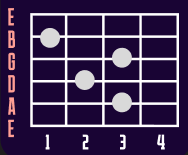
\includegraphics[width=.4\linewidth]{rys02/akord2.2}
	\caption{Wizualna reprezentacja akordu} \label{fig:pageLayout}
\end{figure}

W graficznej reprezentacji akordów pojawiają się określenia: major, minor, sus4, minor7, 7, 9, sus2, maj7, 7\#9, 5. Są to ustalone zbiory nut tworzące poszczególne akordy. Uwzględnienie wszystkich wariacji akordów jest istotne ze względów kompozycyjnych, gdyż poszerza horyzonty muzyków na tworzenie nowych dźwięków, nie ograniczając przy tym ich kreatywności. 

Istotnym aspektem w tworzeniu muzyki jest umiejętność rozpoznawania dźwięków posługując się tylko i wyłącznie słuchem. Posiadanie takiej umiejętności zwykło się nazywać ,,słuchem absolutnym'' dlatego też zawarto w aplikacji trening słuchu, odgrywający losową nutę, którą użytkownik następnie winien odgadnąć.  

\section{Przegląd dostępnych aplikacji}
Poniżej przedstawiono dwie wybrane aplikacje internetowe oferujące materiały oraz narzędzia do nauki gry na gitarze. 

\subsection{Guitar Tuna}
Jedną z większych i cieszących się dużą popularnością aplikacji jest \emph{Guitar Tuna}, oferowana w ramach platformy \cite{Yousician}, dostępna pod adresem: \url{https://yousician.com/guitartuna}). Aplikacja ta jest przeznaczona w głównej mierze na urządzenia mobilne, z ograniczoną ilością funkcji na urządzenia desktopowe. Do oferowanych w niej narzędzi zalicza się: stroik i akordy  (patrz rysunek~\ref{fig:guitartuna}).
\begin{figure}[htb]
	\centering
	\begin{tabular}{ll}
	a) & b) \\
	\vtop{\vskip-2ex\hbox{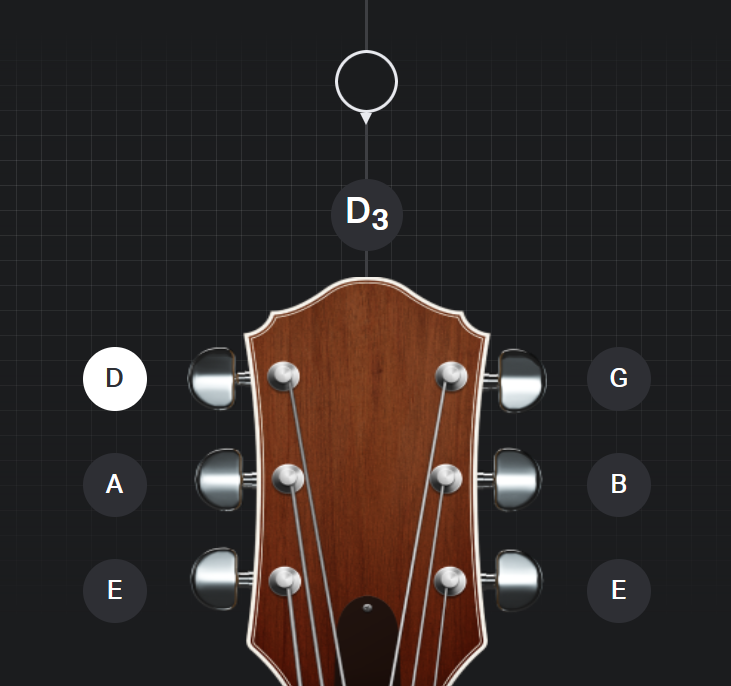
\includegraphics[width=.48\linewidth]{rys02/GTSTROIK}}} &
	\vtop{\vskip-2ex\hbox{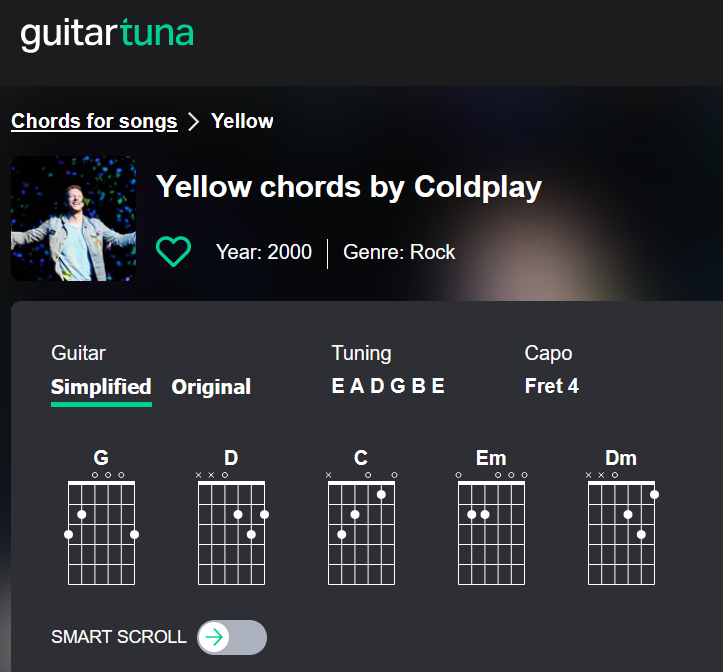
\includegraphics[width=.48\linewidth]{rys02/ChordsGT}}} 
	\end{tabular}
	\caption{Narzędzia dostępne w aplikacji Guitar Tuna: a) stroik, b) sekcja akordów aplikacji} \label{fig:guitartuna}
\end{figure}

\paragraph{Stroik} Stroik gitarowy pokazuje graficznie zagrany ton oraz ,,odległość'' od domniemanej nuty. Narzędzie umożliwia parametryzację polegającą na wyborze docelowej nuty do jakiej chcemy dostroić instrument. Narzędzie umożliwia też wybór instrumentu, wraz z jego graficzną reprezentacją na ekranie i przypisanymi nazwami nut obok odpowiadających pokręteł. Użytkownik do wyboru ma takie instrumenty jak gitara, ukulele, gitara basowa. Dodatkowym atutem jest możliwość wyboru niestandardowych strojeń instrumentów. 

\paragraph{Akordy} Sekcja akordów witryny internetowej jest uboższa aniżeli w aplikacji mobilnej. Narzędzie to daje dostęp do licznych piosenek, przy których przedstawione zostały akordy potrzebne do ich zagrania, wraz z tekstem i przejściami akordów w odpowiednich momentach. Zostało to zrobione statycznie, bez informacji na temat tempa utworu, czy dynamiki przejść pomiędzy granymi akordami. Istnieje tu również myląca funkcja "smart scroll" sugerująca możliwość grania wraz z podkładem grającym w tle, po naciśnięciu przycisku pojawia się jedynie odnośnik do pobrania aplikacji mobilnej.\\


Podsumowując powyższe obserwacje można stwierdzić, że aplikacja sama w sobie jest bardzo przystępna i intuicyjna, największym atutem jest stroik dający dowolność jeżeli chodzi o~używany instrument. Wersja desktopowa jest jednak znacznie okrojona w porównaniu do aplikacji mobilnej, nie znajdziemy tu listy akordów, diagramów skal czy metronomu. 

\subsection{TrueFire}
Aplikacja ta oferuje w większości płatne lekcje i materiały edukacyjne do gry na gitarze:

\begin{itemize}
    \item podkłady muzyczne do gry,
    \item kursy nauki gry poszczególnych stylów muzycznych np. blues, funk czy jazz,
    \item możliwość wykupienia prywatnych lekcji u instruktorów,
    \item transkrypcje znanych piosenek z instrukcjami gry,
\end{itemize}

Poza tym sama witryna zawiera sekcję z narzędziami do nauki (patrz rysunek~\ref{fig:truefire}). Właśnie te narzędzia poddano analizie pod względem użyteczności, czytelności, sposobu przedstawienia poszczególnych elementów.
\begin{figure}[htb]
	\centering
	\begin{tabular}{ll}
	a) & b) \\
	\vtop{\vskip-2ex\hbox{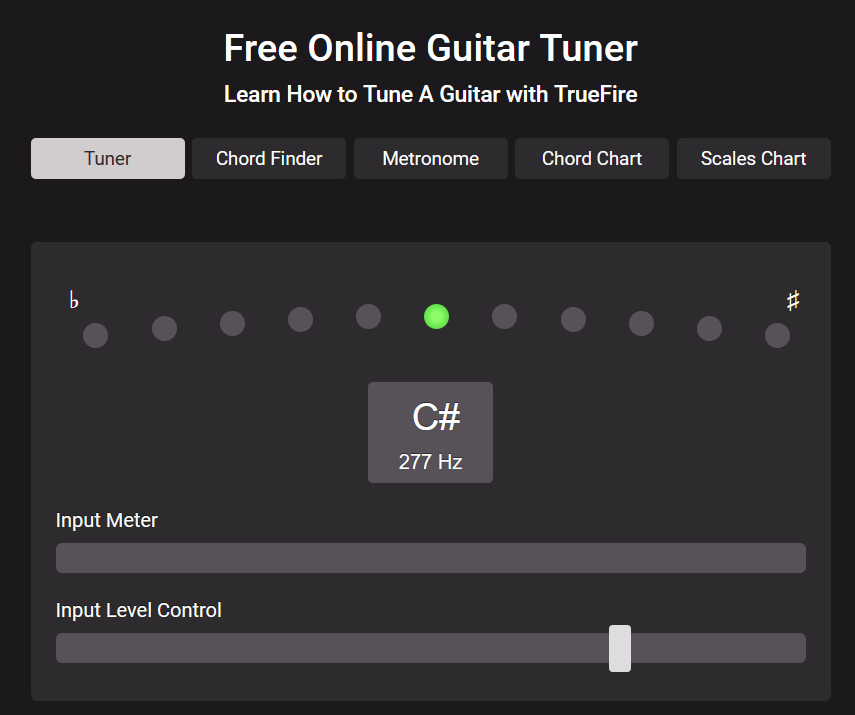
\includegraphics[width=.48\linewidth]{rys02/tuneFireStroik}}} &
	\vtop{\vskip-2ex\hbox{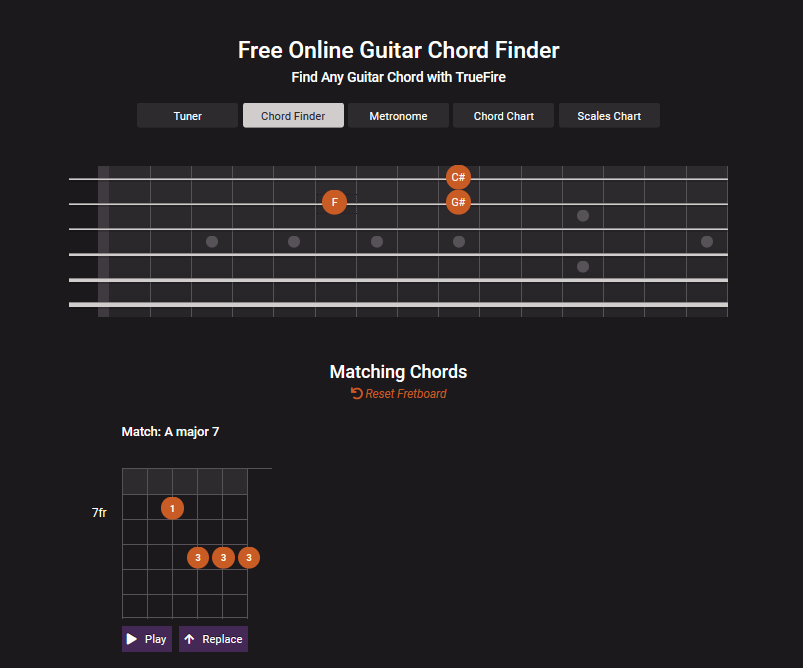
\includegraphics[width=.48\linewidth]{rys02/ChordFinder}}} \\
	c) & d) \\
	\vtop{\vskip-2ex\hbox{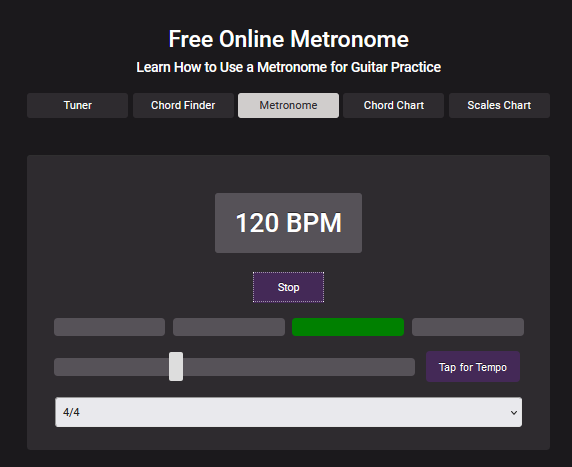
\includegraphics[width=.48\linewidth]{rys02/METRO}}}&
	\multirow{3}{*}{\vtop{\vskip-2ex\hbox{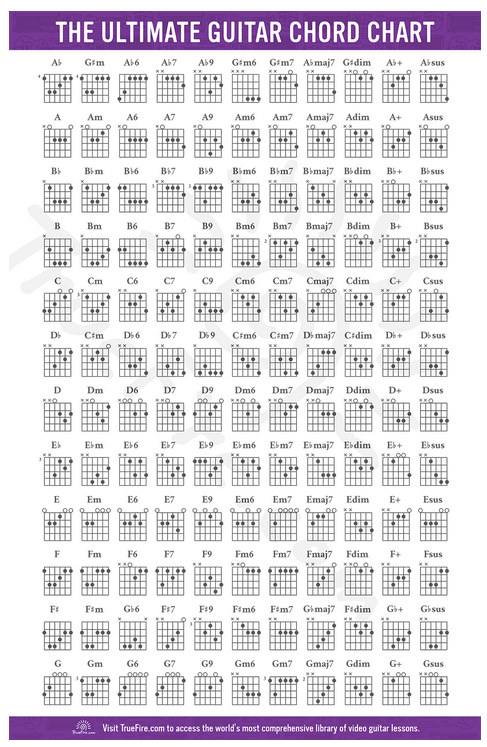
\includegraphics[width=.48\linewidth]{rys02/ChordChart}}}}	\\
	e) & \\
	\vtop{\vskip-2ex\hbox{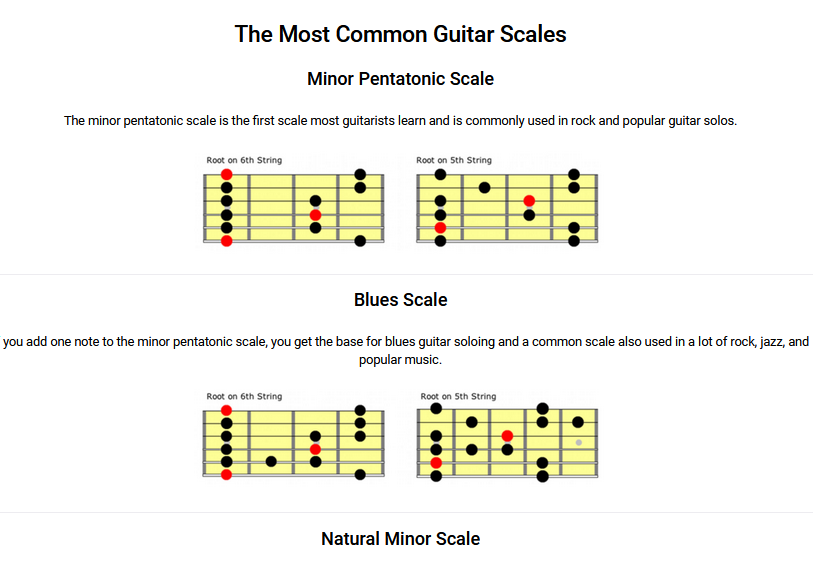
\includegraphics[width=.48\linewidth]{rys02/SKALETF}}} & 
	\end{tabular}
	\caption{Narzędzia dostępne w aplikacji TrueFire: a) stroik, b) eksplorator akordów, c) metronom, d) księga akordów, e) diagram skal} \label{fig:truefire} % TO DO: etykiety nie mogą się powtarzać !!!!!
\end{figure}

\paragraph{Stroik}
Został skonstruowany w sposób bardzo prosty -- rozpoznaje poszczególne dźwięki skali chromatycznej. Zawiera on w sobie \emph{input meter}, będący indykatorem poziomu decybeli dostarczanych do mikrofonu. Ma on również \emph{slider} umożliwiający parametryzację czułości mikrofonu. Samo narzędzie naturalnie umożliwia dostrojenie gitary do poszczególnych dźwięków, może być ono natomiast mało intuicyjne dla początkujących graczy, którzy nie są zapoznani z domyślnym strojeniem strun gitary.

\paragraph{Eksplorator akordów}
Na podstawie zaznaczonych pozycji naciśniętych progów narzędzie to przeszukuje dostępne akordy, wyświetlając najbardziej podobne do zaznaczonych pozycji. Samo narzędzie jest z całą pewnością bardzo kreatywne. Jednak do samej nauki gry wydaje się być mało przydatne. Brak w nim kontekstu przy wyświetlanych znalezionych akordach oraz informacji odnośnie skal, do których sam akord należy. Algorytm dopasowujący nawet w przypadku podania losowych pozycji naciśniętych progów wygeneruje prawidłowe akordy. Może to być mylące dla nowych graczy, którzy błędnie mogą uznać podany przez nich układ jako wpisujący się pod prawidłowe akordy uznawane przez teorię muzyki.



\paragraph{Metronom}
Zaimplementowany jest w sposób prosty, dostarczając wszystkie potrzebne funkcje w jasny i przejrzysty sposób. Dla użytkownika dostępne są funkcje zmiany tempa wybijania poszczególnych bić, możliwość ręcznego ustawienia tempa, oraz dobór metrum z listy 6 dostępnych. Sama realizacja tej funkcji mogłaby zawierać dodatkowo opcję wyboru całych nut, a nie jedynie pół nut i ósemek przy wyborze metrum. Poza tym narzędzie spełnia swoje zadanie.

\paragraph{Księga akordów}

Zaprezentowana została w mało przystępny sposób. Mianowicie w aplikacji prezentowany jest diagram w formie statycznego obrazka, z mało czytelnym podziałem pomiędzy poszczególnymi akordami. Diagram ten jest wadliwy z powodu jego nieczytelności. Z powodu braku kontekstu pod akordami może też być niezrozumiały dla graczy początkujących, jak i średnio zaawansowanych. Same diagramy nie obrazują numeru progu, na którym dany akord ma być grany oraz nie przedstawia nuty odpowiadającej danej strunie.

\paragraph{Diagramy skal}
Przedstawiają one 6 najpopularniejszych skal muzycznych. Brakuje jednak możliwości przeniesienia tych diagramów poprzez gryf, wraz z informacją na temat tego w jakiej skali grany miałby być poszczególny diagram. Jest to rozwiązanie wadliwe, nie dostarczające wystarczająco dużej ilości informacji. \\


Podsumowując powyższe można uznać, że narzędzie dostarcza podstawowych funkcji umożliwiających naukę gry na gitarze, trening rytmu oraz możliwość dostrojenia samego instrumentu. Same funkcje natomiast zostawiają dużo miejsca na rozwój, np.\ przez parametryzację czy też umieszczenie informacji kontekstowych, objaśnienie pewnych sformułowań związanych z pozycjami akordów na gryfie. Narzędzie wyszukiwania akordów na podstawie podanych numerów progów może być mylące. Najbardziej przydatnym narzędziem z zestawienia jest metronom. 

\section{Wnioski}
% DONE: proszę nawiązać trochę do teorii z początku rozdziału
%        potem można przejść do oceny końcowej aplikacji
%        Chodzi o to, by rozdział był spójny - wnioski mają być podsumowaniem całego rozdziału

Przyglądając się wymienionym aplikacjom można dostrzec brak implementacji funkcji koła kwintowego w obydwu rozwiązaniach, będącym ważnym elementem jeżeli chodzi o początki nauki teorii muzyki. Użytkownik podczas korzystania z aplikacji nie ma możliwości zapoznania się z terminami skal muzycznych. Funkcja metronomu pomimo możliwości parametryzacji tempa nie gwarantuje możliwości wyboru wszystkich dostępnych nut wymienionych w pierwszej części rozdziału. Istniejące natomiast narzędzie diagramów skal nie dostarcza wystarczającej ilości informacji, aby uznać je za narzędzie skończone. Biorąc pod uwagę notację gitarową można dostrzec brak ujednoliconego sposobu reprezentacji akordów, wykorzystywane są dwie różne wariacje, przy których również nie znajdziemy pomocy kontekstowej. Do dobrych cech aplikacji można zaliczyć prostotę ich obsługi, zwłaszcza w narzędziu stroika aplikacji Guitar Tuna oraz metronomu Truefire. Do największych wad należy brak kontekstu przy wizualizacji listy dostępnych akordów, oraz ograniczoną ilość możliwości przy wersji desktopowej aplikacji.


